 
%%%%%%%%%%%%%%%%%%%% file cmmr12_template.tex %%%%%%%%%%%%%%%%%%%%%
%
% This is the LaTeX source for the instructions to authors using
% the LaTeX document class 'llncs.cls' for contributions to
% the Lecture Notes in Computer Sciences series.
% http://www.springer.com/lncs       Springer Heidelberg 2006/05/04
%
% It may be used as a template for your own input - copy it
% to a new file with a new name and use it as the basis
% for your article.
%
% NB: the document class 'llncs' has its own and detailed documentation, see
% ftp://ftp.springer.de/data/pubftp/pub/tex/latex/llncs/latex2e/llncsdoc.pdf
%
%%%%%%%%%%%%%%%%%%%%%%%%%%%%%%%%%%%%%%%%%%%%%%%%%%%%%%%%%%%%%%%%%%%


\documentclass[runningheads,a4paper]{llncs}
\usepackage{amssymb}
\setcounter{tocdepth}{3}
\usepackage{graphicx}
\usepackage{url}
\newcommand{\keywords}[1]{\par\addvspace\baselineskip
\noindent\keywordname\enspace\ignorespaces#1}

\pagestyle{headings}

\begin{document}

\mainmatter  % start of an individual contribution

% first the title is needed
\title{ArtDoc - an Experimental Archive and a Tool for Artistic Research}

% a short form shoul2d be given in case it is too long for the running head
\titlerunning{ArtDoc - an Experimental Archive}

% the name(s) of the author(s) follow(s) next
%
% NB: Chinese authors should write their first names(s) in front of
% their surnames. This ensures that the names appear correctly in
% the running heads and the author index.
%
\author{Henrik Frisk \thanks{With acknowledgments to my colleague Jamie Bullock and the Integra project.}}
%
% if the names of the authors are too long for the running head, please use the format: AuthorA et al.
\authorrunning{Henrik Frisk}

% the affiliations are given next; don't give your e-mail address
% unless you accept that it will be published
\institute{Royal College of Music in Stockholm\\ \email{henrik.frisk@kmh.se}}

%
% NB: a more complex sample for affiliations and the mapping to the
% corresponding authors can be found in the file "llncs.dem"
% (search for the string "\mainmatter" where a contribution starts).
% "llncs.dem" accompanies the document class "llncs.cls".
%


\maketitle


\begin{abstract}
ArtDoc is an experimental database and archive for primarily documentation of artistic content. It attempts to address the question of the difficulty of documenting artistic practice in a manner that makes visible the processes in action. The background to this project is discussed and the theory behind the development of open works. Though ArtDoc is still under construction the foundation of the archive is presented. Finally some thoughts on the future of digital documentation systems is discussed.

\end{abstract}


\section{Introduction}
\label{sec:introduction}


What is it to document a musical work? If we assume that one possible means of documenting a work is to record the result, what do we gain, or loose, in the transformation from the work's material reality to its digital representation?\footnote{Digital recordings overshadow almost all analog recording techniques although such documentation is also a possibility.} In this paper I will attempt to approach these questions, and others, from the point of electro acoustic music with or without live parts. 

This research began more than ten years ago and my piece for guitar and electronics that was premiered in Beijing in 2006, \emph{Repetition Repeats all other Repetitions}, has played an important role. Another related project that has contributed to the research is the Integra project \cite{integra}. Integra was a project hosted by Birmingham Conservatoire and funded by the EU, and its initial ambition was to document electronic musical works in a sustainable manner addressing the question of how to avoid that obsolete technology used in these works render them unplayable. \cite{frisk-bullock08,frisk-bull07,bullock06} The method employed in Integra was to collect works from several of the project partner countries and render generic and technology agnostic descriptions of these pieces. In addition, documented software that could be used in order to perform them would also be developed.

The current project is built on the work done in Integra, in particular the research that Jamie Bullock and I did concerning a hierarchy of documentation classes \cite{frisk09,frisk-bullock08}. These were to some extent influenced by the work done in the large European MUSTICA project \cite{bachimont03}. Whereas Integra was a work-centered project--based on the idea that there is a work identity that any performer should adhere to--the current project is rather process oriented. As such it focuses on the elements of the processes that are essential to the creation of the work in new configurations. These two models, the work centered and the development focused, obviously have very different needs when it comes to documentation but also some important overlaps. For the rest of this short paper I will mainly discuss ArtDoc from the point of view of my own artistic work, but it nonetheless rests on the experiences and comparative discussions in the Integra project with its many different types of works (see the sources cited above for reference).

The main difference between these models is that in a traditional view of documentation, in which the work as it was conceived of by its originator, the result, the finished product, is actually a fairly decent means for communicating the intended result, provided that the result is in line with the original intentions. A good recording of a solid interpretation of a work can provide a very good entry in trying to recreate it. This is perhaps less so in the case of a electro acoustic work with live electronic components, but with a score and some instructions a recording provides great help. For a work for which the process of creation plays a conceptually important part, the situation is not only aesthetically substantially different, it is also philosophically different. The work's authenticity lies no longer in the intentions of the originator, but rather in the ears of the listener, or in the hands of the interpreter.\footnote{This discussion could be expanded significantly and it may well be argued that also traditional music is molded by the listener as well as the originator. See \cite{frisk-ost06-2} for an introduction.} How is such a work best documented?

\section{Background}
\label{sec:background}

One of the strong aesthetic tendencies since the 1960s has been to move away from a work centered view of the musical composition and instead move towards a more open work definition. For an open work the final construction of the work may be something that is carried out in, or in preparation for, the performance. Also in traditional works without an inherent openness, however, there has been a significant interest for expanded collaboration between composer and interpreter. The more radical version of openness is what Umberto Eco, who coined the term \emph{Open Work} \cite{eco68} in his seminal book by the same name, calls the work-in-movement,\footnote{Umberto Eco defines the work-in-movement as a more radical kind of open work: ``It invites us to identify inside the category of `open' works a further, more restricted classification of works which can be defined as `works in movement', because they characteristically consist of unplanned or physically incomplete structural units.'' \cite{eco68}} where the work is a latent, or prospective, possibility. For such a work, composing consists of supplying raw material for a work, delivering a potential work rather than a finished one. In the collaborative project mentioned above we departed from Umberto Eco's reasoning and developed an artistic method that leaned strongly on the idea of the work as a continuously developing field of possibilities. What started as a fairly standard composition for guitar and electronics, \emph{Repetition Repeats all other Repetitions} developed into a work-in-movement whose work identity was located in change rather than fixity. \cite{eco68,frisk08} In a few articles published early in the process we discuss how our view on the work developed in the process. \cite{frisk-ost06,frisk-ost06-2}

The development of \emph{Repetition Repeats all other Repetitions} coincided with the development of a documentation database for the Integra project. As such it invited interpreters to create their own work out of an assembly of segments that could be combined in a number of different manners. Had these segments only consisted of written instructions in musical notation the challenge of creating this particular work's documentation may have been slightly easier. However, the documentation had to contain not only all previous versions and their modes of construction, but also all the different parts in terms of electronic sounds (sound files, software for interaction, DSP processes for altering the acoustic sounds, etc.). The idea of a documentation database for the piece appeared as a sensible solution. Although the database developed in the Integra project was mainly designed for the preservation of works, its structure turned out to be apt also for the current context.

The ruling principle for this project is that there is no such thing as an ultimate performance, or rendering of the work. The work is not a singleton but a realizable potential. Each performance of each work makes possible a new work and this development is the true nature of the work identity. It simultaneously makes impossible an exact repetition. How can this incremental process be documented to allow the work-in-movement to continue to move and not just repeat itself? Is an archive that archives in order to allow for change possible or even desirable?

In the field of artistic research the topic of documentation is of great importance. Given the novelty of the field it may even be relevant to ask what artistic research data actually consist of. To add to the complexity, in a research context there is the need to collect material necessary for a systematic investigation of the process. In addition, to research the process of creation there is a need to develop systems that surfaces and makes visible the activities that relate to the work creation. The issue may be divided into several subtopics but first and foremost it is important to distinguish between the gathering of research data, and the documentation of the result. Even if the result may be easily documented, the data, the processes that led to the result, is commonly of central importance to the research process. How can the integrity of the data be preserved in an artistic research project that may contain a number of different kinds of data, as well as raw material from the artistic process? 

\section{Method}
\label{sec:method}

One preliminary, however inconclusive, way to understand this question is that in artistic research the material basis of the artistic practice may be both data and result. The way in which either could be represented in the research is however largely still an unsolved issue. Particularly in the context of performative arts and music. One point of departure for the research presented here is that it is necessary to critically examine the relations between artistic practice in music and its possible representations in various forms for archives. This, and the more general question of the tendency of any archive to, so to say, write itself, is discussed in an forthcoming article in a thematic issue on digitization in The Swedish Journal of Music Research \cite{frisk16}.

An archive of musical material most often archives representations of musical content, and to be meaningful such archive has to go beyond a mere collection of resources. An archived score is relatively easy to represent accurately but is a poor representation of the actual music. A recording of a performance is an accurate representation of the sound but a poor representation of the material performance. Furthermore, within the category of musical recordings, there are a number of different methods to record and archive a performance most, if not all, of which are reductions of the materiality of the performance when adapted to the archivable documentation/representation format. How, then, may an archive for artistic research and artistic practice be structured?

Conveniently, in the case of \emph{Repetition Repeats all other Repetitions} the research data and the artistic practice coincide to a significant degree. Hence, the method for exploring what are the efficient means for archiving data coincides with the artistic methods used in the creation of the development of the piece. It is the development of the piece that can give answer to the question of what is required of the archive. Leaning on the previously mentioned work in the Integra project a set of documentation classes was developed and tried in numerous contexts (see Fig.~\ref{fig:example}).

\begin{figure}
\centering
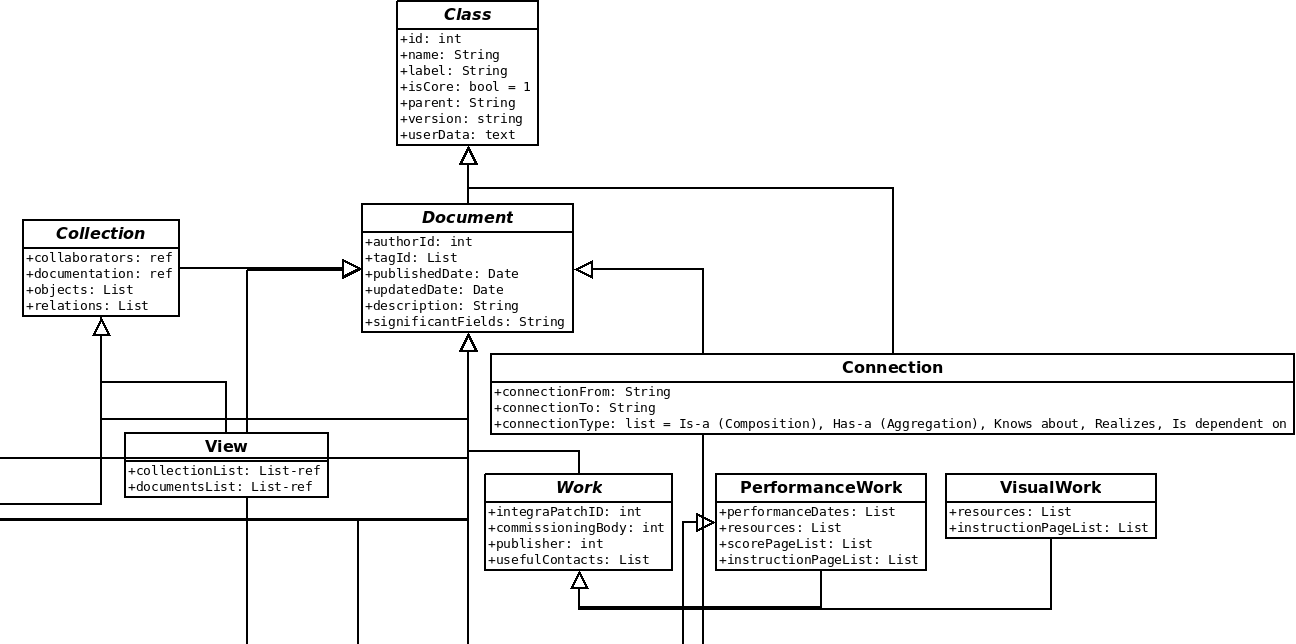
\includegraphics[height=6.2cm]{img/classdiagramC.png}
\caption{A part of the diagram for the latest version of the class hierarchy for the documentation system ArtDoc. All classes inherit the class \emph{Document} that inherits the base class \emph{Class}. This allows for new and ever more specialized classes to be easily added.}
\label{fig:example}
\end{figure}

\section{The Archive}
\label{sec:archive}
One of the fundamental properties of this experimental documentation archive is that the most important class is the \emph{Connection}. It defines a two way connection between two related instances. This way chains of instances can portray a semantic web, both in the ways that the connections give meaning to instances, and in the way that one instance can be understood in the number of connections it has. In this way, once the raw data has been entered and connections are made, the archive becomes a method in itself. Furthermore, connections can point to specific points in instances, such as a particular point in time.

All classes have a corresponding XML description which acts as a template for all instances. The following is an example of the \emph{Connection} class, as is shown below.

\medskip

\noindent
{\it Example of a class definition}
\begin{verbatim}
<Class xmlns:xsi="http://www.w3.org/2001/XMLSchema-instance">
    <class-name>Connection</class-name>
    <parent>Class</parent>
    <class-description>A child class to Document describing any kind of 
     connection between two nodes within the system. The id of the 
     connected classes are the references
    </class-description>
    <documentation/>
    <attributes>
        <connection-from type="Ref" ref-class="Document" 
                         desc="Connection from" edit="1" 
                         required="1"/>
        <connection-to type="Ref" ref-class="Document" 
                       desc="Connection to" edit="1" 
                       required="1"/>
        <connection-type type="select" desc="Type of connection" 
                         edit="1" required="1"/>
    </attributes>
</Class>
\end{verbatim}

Apart from the \emph{Connection} class the \emph{View} class is also important. With it the user may group instances together in \emph{Collection}s and create independent views. For example, a selection of videos from a performance can be grouped together into a view.
The design principle has been to keep classes small and generic. It should be possible to add new classes to the structure simply by adding a new class definition. The structure that the class diagram shows above, however, does not currently have a working implementation. A test was implemented and presented in \cite{frisk08} and a working web based beta version is expected in the August 2017. 

\section{Discussion}
\label{sec:discussion}
The question of how to best document the intense creative forces that digital technology allows for is without doubt one of the important ones in the upcoming decades. On the one hand there is the risk that the nearly ubiquitous digital domain negatively influences the willingness to invest in an active listening process. Though there is little that actually points in this direction\footnote{If anything, listening to live music appears to have increased in urban areas.} the convenience of online music services that delivers exactly the music we think we want to hear is intimidating at times. On the other hand we now have access to incredible tools that may make visible aspects of musical composition and interpretation in ways that has not previously been possible. This latter aspect is what ArtDoc attempts to provide some initial access to. 

If it proves effective at this task there are a number of ways in which it can be expanded. For example, currently ArtDoc is largely a single user version where users are offered to document their own work. However, due to its modularity it would be relatively simple to add a system of permissions allowing a network of users to interact with each other. The functionality that the classes \emph{Collection} and \emph{View} offers can with some modification turn the archive into a presentation tool or even a performance tool in its own right.

%\subsubsection*{Acknowledgments.} The heading should be treated as a
%subsubsection heading and should not be assigned a number.

%&\section{The References Section}\label{references}


\begin{thebibliography}{99}
\bibitem{bachimont03}
B~Bachimont, J.-F. Blanchette, A~Gerzso, A~Swetland, O~Lescurieux,
  P~Morizet-Mahoudeaux, N~Donin, J~Teasley.: Preserving interactive digital music: a report on the MUSTICA
  research initiative. Proceedings. Third International Conference on Web Delivering
  of Music. WEDELMUSIC, (2003)

\bibitem{bullock06}
Bullock, J., Coccioli, L.:
Modernising musical works involving Yamaha DX-based synthesis: a
  case study. Organised Sound, 11(3), (2006)

\bibitem{frisk-bull07}
Bullock, J., Frisk, H.: libIntegra: A System for Software-Independent Multimedia Module
  Description and Storage. In Proceedings of the International Computer Music Conference
  2007, Copenhagen, Denmark. (2007)

\bibitem{frisk09}
Bullock, J.,Frisk, H.: An object oriented model for the representation of temporal data in
  the Integra framework. In ICMC. (2009)

\bibitem{frisk-bullock08}
Bullock, B., Frisk, H., Coccioli, L.: Sustainability of `Live Electronic' Music in the Integra Project.
In The 14th IEEE Mediterranean Electrotechnical Conference
  Proceedings, Ajaccio, Corsica. (2008)

\bibitem{eco68} Eco, U.: The Open Work. Hutchinson Radius. (1968)

\bibitem{frisk08} Frisk, H.: Improvisation, Computers, and Interaction: Rethinking Human-Computer Interaction Through Music. PhD thesis, Malm{\{}{\"{o}}{\}} Faculty of Fine and Performing Arts,
  Lund University. (2008)

\bibitem{frisk16} Frisk, H.: The Archive the writes itself, Swedish Journal of Music Research. In print. (2017)

\bibitem{frisk-ost06}
Frisk, H., Östersjö, S.: Negotiating the Musical Work. An empirical study.
In Proceedings of the International Computer Music Conference
  2006, 242--249. ICMA, San Francisco, Calif.: Computer Music Assoc.,
  (2006)

\bibitem{frisk-ost06-2}
Frisk, H., Östersjö, S.: Negotiating the Musical Work. An empirical study on the inter-relation between composition, interpretation and performance.
In Proceedings of EMS -06, Beijing. Terminology and Translation. Electroacoustic Music Studies, EMS. (2006)

\bibitem{frisk-ost13}
Frisk, H., Östersjö, S.: Beyond Validity: claiming the legacy of the artist-researcher.
STM, 1--17, 2013.

\bibitem{integra} IntegraLab, \url{http://integra.io/}

\end{thebibliography}



\end{document}
